Программа <<WhoseCppCode>>, разработанная в ходе работы, состоит из двух основных частей:
\begin{itemize}
 \item программного модуля, реализующего все необходимые функции для сбора, анализа и обработки данных, 
а также построения модели классификации авторов исходного кода, описанной в разделе~\ref{modeling};
 \item программного интерфеса на основе технологии Jupyter Notebook~\cite{jupyter}, предназначенного 
 для визуализации полученных в ходе классификации результатов, сбора необходимых данных с ресурса GitHub~\cite{GitHub},
 построения матрицы объектов-признаков на основе входных данных, проведения вычислительных экспериментов.
\end{itemize}

Программный модуль реализован на языке прораммирования высокого уровня Python с использованием следующих 
программных библиотек:
\begin{itemize}
 \item Scikit-Learn~\cite{scikit} --- open-source библиотека для машинного обучения: классификации, регрессии, кластеризации и т.д.
 \item Plotly~\cite{plotly} --- графическая Python-библиотека для построения интерактивных графиков, таблиц, диаграмм.
 \item Numpy~\cite{numpy} --- библиотека для научных вычислений, предоставляющая методы работы с большими массивами данных.
 \item Scipy~\cite{scipy} --- предоставляет среду для проведения математических и научных вычислений.
 \item Pandas~\cite{pandas} --- open-source библиотека, предназначенная для анализа данных.
 \item Ipywidgets~\cite{widgets} --- интерактивные HTML виджеты для Jupyter Notebook.
\end{itemize}

Интерфейс основан на веб-технологиях, может использоваться для демонстрации возможностей
программ на языке Python. Библиотека Jupyter Notebook, с помощью которой был реализован
данный интерфейс, была выбрана за счет ряда преимуществ:
\begin{itemize}
 \item является свободным ПО;
 \item поддерживает множество языков программирования;
 \item позволяет хранить вместе код, изображения, комментарии, формулы и графики;
 \item не требует знаний и применения веб-технологий, таких как CSS, HTML, JavaScript;
 \item может быть запущен на любом сервере, необходим только доступ по ssh/http;
 \item позволяет экспортировать код и сам блокнот в любом формате;
 \item предназначена для демонстрации разработок на языке Python (в основном в машинном обучении).
\end{itemize}

Основной модуль программы <<WhoseCppCode>> может быть использован отдельно от Jupyter Notebook 
при разработке различного рода программ, систем и интерфейсов лицами, заинтересованными в задаче
классификации программистов.

Диаграмма действий в нотации UML, описывющая основной алгоритм работы программы <<WhoseCppCode>>
представлена на рисунке~\ref{flowchart:flowchart}, примеры ввода и вывода данных в интерфейсе Jupyter 
Notebook --- на рисунках~\ref{main_module:main_module}, \ref{newplot:newplot} и~\ref{newplot2:newplot2}.

\begin{figure}[h!]
\center{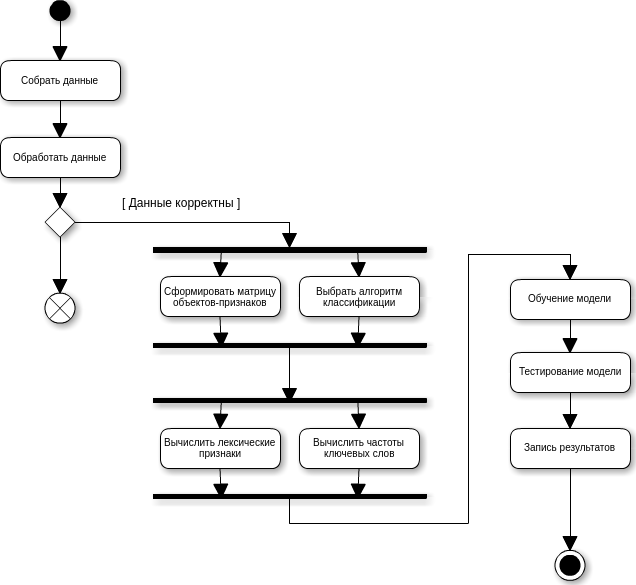
\includegraphics[width=0.9\linewidth]{flowchart}}
\caption{ Диаграмма действий алгоритма работы программы <<WhoseCppCode>> }
\label{flowchart:flowchart}
\end{figure}


\begin{figure}[h!]
\center{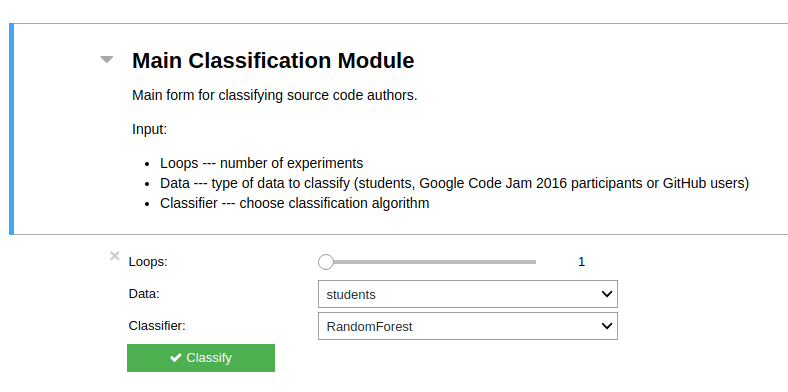
\includegraphics[width=0.7\linewidth]{main_module}}
\caption{ Вид основной формы программного интерфейса }
\label{main_module:main_module}
\end{figure}

\begin{figure}[h!]
\center{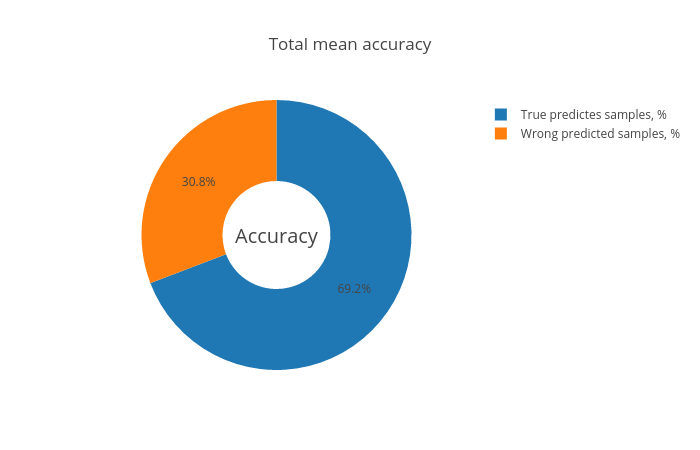
\includegraphics[width=0.7\linewidth]{newplot}}
\caption{ Вывод диаграммы результатов классификации }
\label{newplot:newplot}
\end{figure}

\begin{figure}[h!]
\center{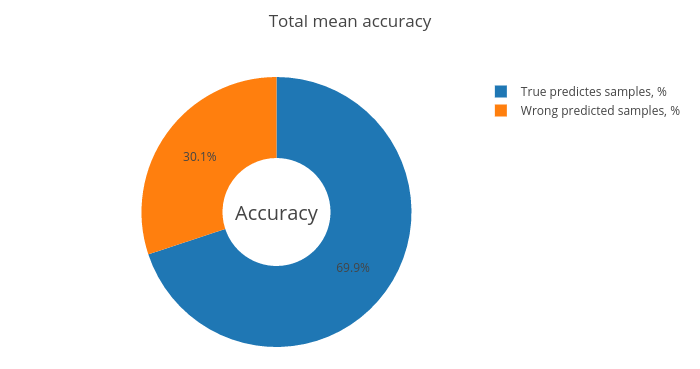
\includegraphics[width=0.7\linewidth]{newplot2}}
\caption{ Пример вывода диаграммы для средней точности классификации }
\label{newplot2:newplot2}
\end{figure}

% Описание функций, реализованных в основном модуле программы, а также
% примеры ввода и вывода данных в интерфейсе Jupyter Notebook представлены в приложениях Г и Д соответственно. 

